\documentclass{standalone}
\usepackage{tikz}

\usetikzlibrary{calc,intersections}


\begin{document}

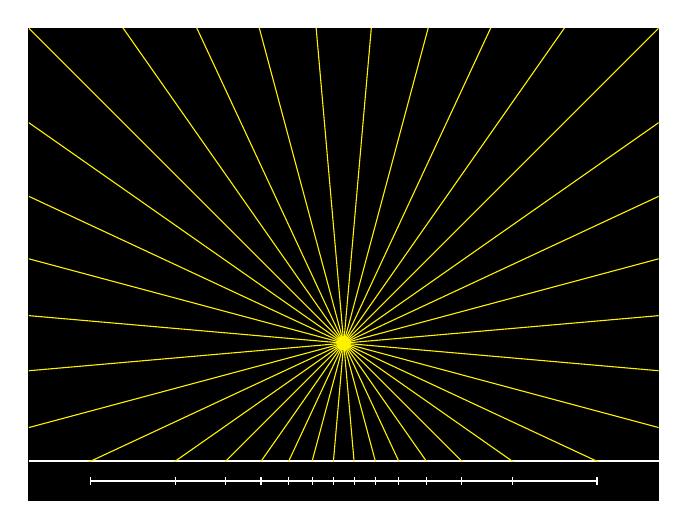
\begin{tikzpicture}
  \draw[fill=black,black] (-4,-2) rectangle (4,4);
  \draw[fill=yellow] (0,0) circle [radius=0.1cm];
  \draw[thick,white,name path=wall] (-4,-1.5) -- (4,-1.5);

  \begin{scope}
    \path[clip] (-4,-1.5) rectangle (4,4);

    \foreach[count=\i] \x in {-95,-85,...,260} {
      \draw[thin,yellow,name path={ray}] (0,0) -- (\x:8);
      \path[name intersections={of=wall and ray,by=h\i}];
    }
  \end{scope}

  \draw[white] let \p1=(h8), \p2=(h31) in ($ (\p1) - (0,0.25) $) -- ($ (\p2) - (0,0.25) $);
  \foreach \i in {1,...,36} {
    \draw[white] ($ (h\i) - (0,0.3) $) -- ($ (h\i) - (0,0.2) $);
  }
\end{tikzpicture}

\end{document}